\let\negmedspace\undefined
\let\negthickspace\undefined
\documentclass[journal]{IEEEtran}
\usepackage[a5paper, margin=10mm, onecolumn]{geometry}
%\usepackage{lmodern} % Ensure lmodern is loaded for pdflatex
\usepackage{tfrupee} % Include tfrupee package

\setlength{\headheight}{1cm} % Set the height of the header box
\setlength{\headsep}{0mm}     % Set the distance between the header box and the top of the text

\usepackage{gvv-book}
\usepackage{gvv}
\usepackage{cite}
\usepackage{amsmath,amssymb,amsfonts,amsthm}
\usepackage{algorithmic}
\usepackage{graphicx}
\usepackage{textcomp}
\usepackage{xcolor}
\usepackage{txfonts}
\usepackage{listings}
\usepackage{enumitem}
\usepackage{mathtools}
\usepackage{gensymb}
\usepackage{comment}
\usepackage[breaklinks=true]{hyperref}
\usepackage{tkz-euclide} 
\usepackage{listings}
% \usepackage{gvv}                                        
\def\inputGnumericTable{}                                 
\usepackage[latin1]{inputenc}                                
\usepackage{color}                                            
\usepackage{array}                                            
\usepackage{longtable}                                       
\usepackage{calc}                                             
\usepackage{multirow}                                         
\usepackage{hhline}                                           
\usepackage{ifthen}                                           
\usepackage{lscape}
\begin{document}

\bibliographystyle{IEEEtran}
\vspace{3cm}

\title{1.5.5}
\author{EE25BTECH11017 - CHOLLANGI MAHESH}
% \maketitle
% \newpage
% \bigskip
{\let\newpage\relax\maketitle}

\renewcommand{\thefigure}{\theenumi}
\renewcommand{\thetable}{\theenumi}
\setlength{\intextsep}{10pt} % Space between text and floats


\numberwithin{equation}{enumi}
\numberwithin{figure}{enumi}
\renewcommand{\thetable}{\theenumi}


\textbf{Question}:\\
\begin{enumerate}
\item Find the coordinates of the point which divides the line segment joining the points$\vec{A}$ $\brak{7,-1}$ and $\vec{B}$ $\brak{-3, -4}$ in the ratio $2 : 3$ \dots.
\end{enumerate}

\quad

\textbf{Solution:}
Let us consider the coordinates of $\vec{P}$  on $\vec{AB}$ such that $\vec{AP:PB}=2:3 ,$ where coordinates of A = $\myvec{7\\-1}$ and B are $\myvec{-3\\-4}$ are 

\begin{align}
\vec{P}=\frac{k(\vec{B})+(\vec{A})}{k+1}\\
\end{align}
Here according to problem value of k is 2/3\\
\begin{align}
\vec{P}=\frac{2(\vec{B})+3(\vec{A})}{5}=\frac{2\myvec{-3\\-4}+3\myvec{7\\-1}}{5}=\frac{\myvec{15\\-11}}{5}\\
\end{align}
\begin{align}
\vec{P}=\myvec{3\\-11/5}
\end{align}
Hence the coordinates of $\vec{P}$ are $\brak{3,-11/5}$
\begin{figure}
    \centering
    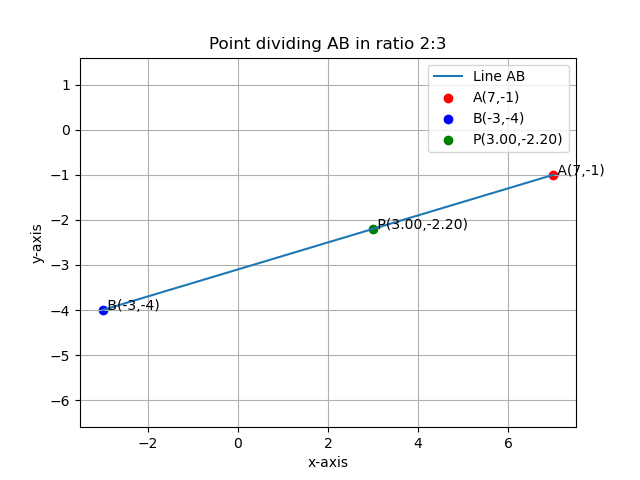
\includegraphics[width=0.7\linewidth]{figs/plot.png}
    \caption{Stem plot of y\brak{n}}
    \label{stemplot}
\end{figure}
\end{document}  
